
\definecolor{c808080}{RGB}{128,128,128}
\definecolor{c999999}{RGB}{153,153,153}


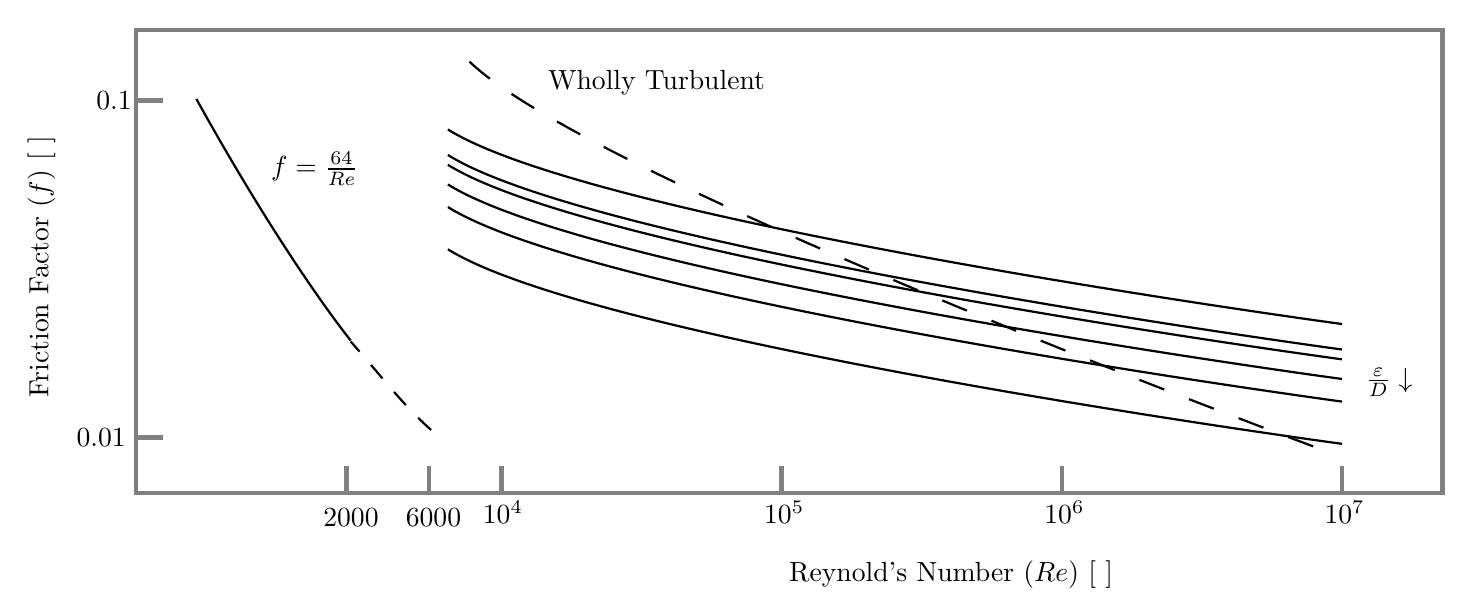
\begin{tikzpicture}[y=0.80pt, x=0.8pt,yscale=-1, inner sep=0pt, outer sep=0pt]
\begin{scope}[shift={(0,-782.35975)}]
  \path[draw=c808080,miter limit=4.00,line width=1.600pt,rounded corners=0.0000cm]
    (70.4594,794.8260) rectangle (660.5406,1003.8935);
  \path[draw=c808080,line join=miter,line cap=butt,miter limit=4.00,line
    width=1.600pt] (70.4594,826.6674) -- (82.4417,826.6674);
  \path[draw=c808080,line join=miter,line cap=butt,miter limit=4.00,line
    width=1.600pt] (70.4594,978.8864) -- (82.4417,978.8864);
  \path[draw=c808080,line join=miter,line cap=butt,miter limit=4.00,line
    width=1.600pt] (165.3964,1003.8935) -- (165.3964,991.9113);
  \path[draw=c808080,line join=miter,line cap=butt,miter limit=4.00,line
    width=1.600pt] (202.6331,1003.8935) -- (202.6331,991.9113);
  \path[draw=c808080,line join=miter,line cap=butt,miter limit=4.00,line
    width=1.600pt] (235.4615,1003.8935) -- (235.4615,991.9113);
  \path[draw=c808080,line join=miter,line cap=butt,miter limit=4.00,line
    width=1.600pt] (362.0178,1003.8935) -- (362.0178,991.9113);
  \path[draw=c808080,line join=miter,line cap=butt,miter limit=4.00,line
    width=1.600pt] (488.5740,1003.8935) -- (488.5740,991.9113);
  \path[draw=c808080,line join=miter,line cap=butt,miter limit=4.00,line
    width=1.600pt] (615.1302,1003.8935) -- (615.1302,991.9113);
  \path[fill=c999999] (52.4142,830.90668) node[above right] (text3839) {0.1};
  \path[fill=c999999] (43.50795,983.12561) node[above right] (text3843) {0.01};
  \path[fill=c999999] (154.96872,1019.1635) node[above right] (text3847) {$2000$};
  \path[fill=c999999] (192.2054,1019.1635) node[above right] (text3847-2)
    {$6000$};
  \path[fill=c999999] (227.0338,1017.9819) node[above right] (text3847-2-5)
    {$10^{4}$};
  \path[fill=c999999] (354.08807,1017.9819) node[above right] (text3847-2-5-1)
    {$10^{5}$};
  \path[fill=c999999] (480.64429,1017.9819) node[above right] (text3847-2-5-11)
    {$10^{6}$};
  \path[fill=c999999] (607.2005,1017.9819) node[above right] (text3847-2-5-2)
    {$10^{7}$};
  \path[fill=c999999] (365.38672,1047.0343) node[above right] (text3932)
    {Reynold's Number ($Re$) [ ]};
  \path[cm={{0.0,-1.0,1.0,0.0,(0.0,0.0)}},fill=c999999] (-961.04724,21.434233)
    node[above right] (text3932-1) {\rotatebox{90}{Friction Factor ($f$) [ ]}};
  \path[shift={(0,782.35975)},draw=black,line join=miter,line cap=butt,line
    width=0.800pt] (97.6331,43.6686) .. controls (138.4615,117.3373) and
    (167.3227,152.7507) .. (167.3227,152.7507);
  \path[shift={(0,782.35975)},draw=black,dash pattern=on 6.40pt off 6.40pt,line
    join=miter,line cap=butt,miter limit=4.00,line width=0.800pt]
    (203.6498,193.1651) .. controls (190.4531,181.4029) and (181.9179,169.6407) ..
    (167.3227,153.2169);
  \path[shift={(0,782.35975)},draw=black,line join=miter,line cap=butt,line
    width=0.800pt] (211.2426,92.4852) .. controls (279.5858,135.0888) and
    (615.0888,180.3550) .. (615.0888,180.3550);
  \path[draw=black,line join=miter,line cap=butt,line width=0.800pt]
    (211.2426,864.6379) .. controls (279.5858,907.2414) and (615.0888,952.5077) ..
    (615.0888,952.5077);
  \path[draw=black,line join=miter,line cap=butt,line width=0.800pt]
    (211.2426,855.7621) .. controls (279.5858,898.3657) and (615.0888,943.6319) ..
    (615.0888,943.6319);
  \path[draw=black,line join=miter,line cap=butt,line width=0.800pt]
    (211.2426,839.8095) .. controls (279.5858,882.4130) and (615.0888,927.6793) ..
    (615.0888,927.6793);
  \path[draw=black,line join=miter,line cap=butt,line width=0.800pt]
    (211.2426,851.3243) .. controls (279.5858,893.9278) and (615.0888,939.1941) ..
    (615.0888,939.1941);
  \path[shift={(0,782.35975)},draw=black,dash pattern=on 9.60pt off 9.60pt,line
    join=miter,line cap=butt,miter limit=4.00,line width=0.800pt]
    (221.0059,26.8047) .. controls (276.9231,80.9467) and (609.7633,203.4320) ..
    (609.7633,203.4320);
  \path[draw=black,line join=miter,line cap=butt,line width=0.800pt]
    (211.2426,893.9278) .. controls (279.5858,936.5314) and (615.0888,981.7976) ..
    (615.0888,981.7976);
  \path[shift={(0,782.35975)},fill=black] (256.50888,41.89349) node[above right]
    (text4022) {Wholly Turbulent};
  \path[fill=black] (131.36095,865.08167) node[above right] (text4026)
    {$f=\frac{64}{Re}$};
  \path[fill=black] (625.73962,960.49585) node[above right] (text4030)
    {$\frac{\varepsilon}{D} \downarrow$};
\end{scope}

\end{tikzpicture}
